\section{Generalization}\label{sec:generalization}
\begin{comment}
    One of the cornerstones in designing efficient ML systems is accurately estimating the performance of learning algorithms. Among various theoretical frameworks, the theory of uniform convergence of empirical quantities to their mean, as pioneered by Vapnik, provides a robust foundation for understanding risk (or generalization error). By examining empirical accuracy measurements in conjunction with complexity metrics (e.g., the Vapnik–Chervonenkis dimension or the fat-shattering dimension), one can systematically gauge how well a learned model will perform on previously unseen data. \cite{Vapnik1982,Alon1997}

In practice, these theoretical insights are put into operation by employing suitable error measures, which quantify how closely a model’s predictions align with ground truth. 
\end{comment}
In this project, we follow the approach detailed in our previous milestone and evaluate our models using accuracy, precision, recall, F1-Score, and AUC-ROC. \cite{Ammar2024}

Precision helps minimize the incorrect flagging of benign comments as toxic, whereas recall focuses on reducing missed detections of actual toxic content. F1-Score balances these two metrics, making it particularly suitable for scenarios with class imbalance. Meanwhile, AUC-ROC provides a holistic view by measuring the model’s capacity to distinguish between positive and negative classes across various decision thresholds.

Despite the utility of all these metrics, we place special emphasis on the F1-Score for the toxic class, given its effectiveness with imbalanced datasets. Other measures often yield satisfactory results across different models, but it is precisely on this toxic class F1 that the better-performing approaches distinguish themselves. These considerations enable a nuanced understanding of our model's strengths and weaknesses, especially when compared to baseline classifiers.

\subsection{Empirical estimates}
The generalization error was estimated using the Civil Comments test dataset for all baseline models and BERT, as illustrated in \cref{fig:performance}. The BERT configuration follows the setup described in \cref{subsec:chosen_configuration}. Among the baseline models, Naïve Bayes exhibited the weakest performance, although it remained computationally efficient. In contrast, SVM and logistic regression achieved comparable results, with an F1-score of (at least) 0.61 for the toxic class and an AUC-ROC of 0.94. 

BERT outperformed these baselines significantly, particularly in the F1-score for the positive class, reaching 0.7, and demonstrated superior AUC-ROC performance with a score of 0.98. These empirical estimates are considered reliable, as the results obtained from the test dataset closely align with those observed on the validation dataset, supporting the consistency and robustness of the model's performance across different data splits.

\begin{figure}[ht]
    \centering
    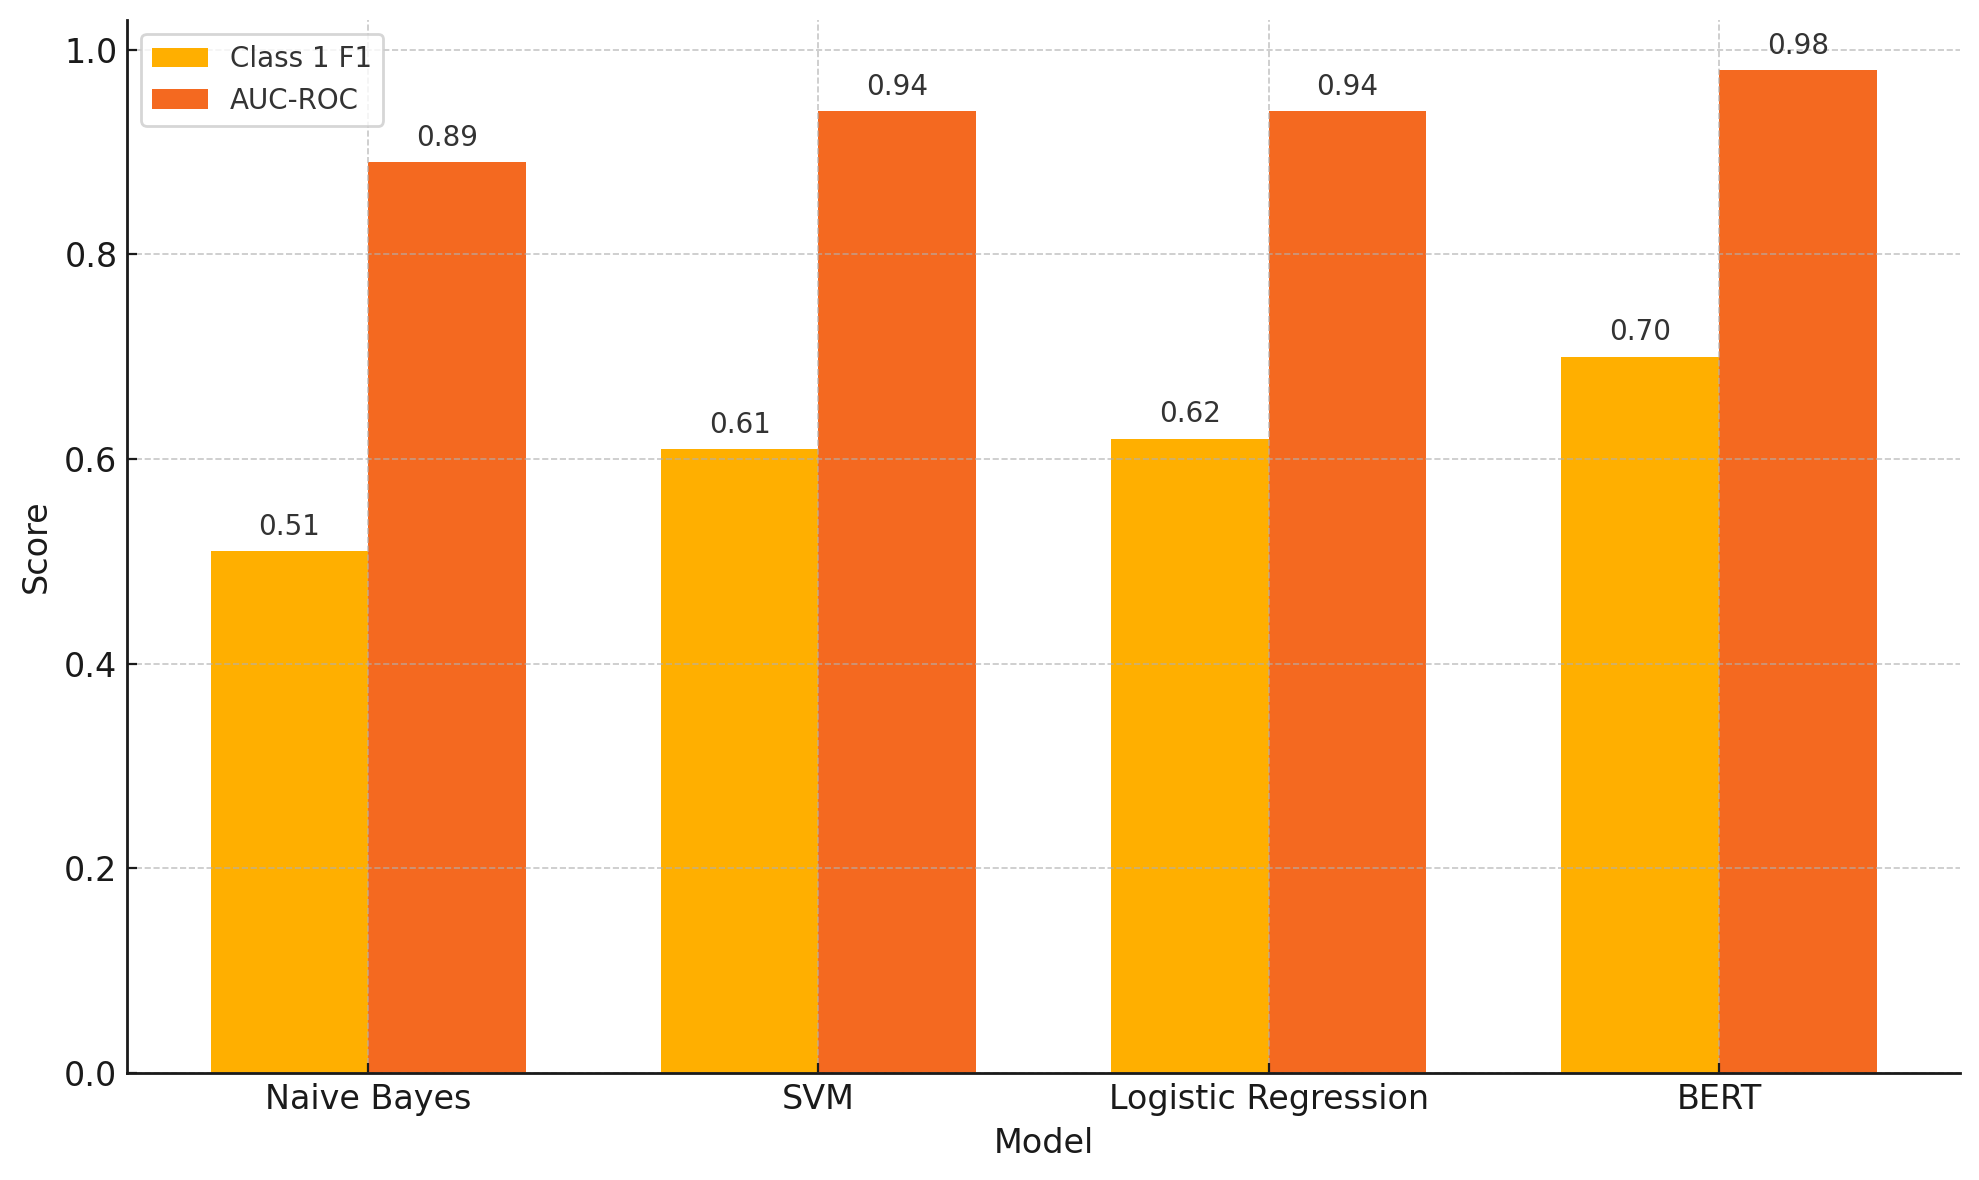
\includegraphics[width=0.6\textwidth]{./figures/performance_compare.png}
    \caption{Models' performance on the Civil Comments test dataset.}
    \label{fig:performance}
\end{figure}

\subsection{Test cases}
For evaluating our model and baselines, we utilize precision, recall (in F1), and AUC-ROC as error measures. However, these metrics alone are insufficient for identifying the best or worst individual predictions. To address this, we introduce a confidence score defined as follows:

\begin{equation}
    C = \max(p, 1 - p),
\end{equation}

\noindent where $p$ is the probability of the positive class output by the model. This score ranges from 0.5 to 1, with higher values indicating greater confidence in the model's prediction. Using this measure, we classify predictions into three categories: low (0.5-0.66), moderate (0.66-0.85), and high (0.85-1) confidence predictions.

\Cref{fig:confidence_comparison} in the appendix illustrates the distribution of confidence scores for the baseline method and BERT. The left column shows the confidence score distribution, while the right column highlights the incorrect predictions. Both models exhibit a significant concentration of predictions in the high-confidence range. Notably, low-confidence predictions are rare, suggesting limited expression of uncertainty by both methods.

Furthermore, we observe that the baseline model produces a nearly uniform distribution of confidence scores for false predictions while high confidence scores for false predictions become less frequent in BERT. This indicates that SVM lacks confidence in its predictions and has a limited ability to separate correct from incorrect classifications. BERT, on the other hand, demonstrates a better grasp of uncertainty and reflects a more realistic confidence assessment. Its calibration is superior to the baseline model, even if it still produces false predictions. To better understand its performance in high and low confidence ranges, we analyze examples of high- and low-confidence predictions.

\subsubsection{High confidence}
This category encompasses both the best predictions (high confidence, correct classification) and the worst predictions (high confidence, incorrect classification). Representative examples of correct high-confidence predictions are listed in \cref{tab:confident_correct}, while incorrect high-confidence predictions appear in \cref{sec:examples}.

The distinction between toxic and non-toxic comments is primarily determined by linguistic features and the model's confidence scores. Non-toxic comments typically exhibit polite or neutral language—often expressing gratitude, affirmation, or sharing information—and are associated with exceptionally high confidence scores, indicating strong certainty in their classification. In contrast, toxic comments frequently feature hostile, insulting, or profane language, accompanied by slightly lower confidence scores. This discrepancy reflects the greater lexical and contextual variability inherent in toxic expressions. Additionally, toxic comments are often shorter and more direct, simplifying their identification but also introducing challenges in detecting subtle forms of toxicity, such as sarcasm or coded language. Notably, for this analysis, the top three high-confidence toxic comments were not included because many top predictions were highly repetitive, consisting of variations of simple insults (e.g., “idiot”). These observations highlight the model’s reliance on explicit linguistic cues for toxicity detection while suggesting opportunities for improving its ability to capture more nuanced harmful expressions.

To gain deeper insights into the model's performance, we take a closer look at some of the incorrect predictions. While “stupid” is clearly a false negative (likely due to the Unicode emoji) and “damn right” is a false positive, the toxicity of “Total Clueless Jerk” and “Flat earther moron.” can be debated. Both have relatively high (0.31 and 0.48) ground-truth toxicity scores but do not surpass the threshold of 0.5. The other false negatives are lengthy comments, with toxic language near the end; this suggests that the 128-sequence-length limit may contribute to misclassification.

\begin{table}[htbp]
    \centering
    \caption{Correct high-confidence predictions}
    \label{tab:confident_correct}
    \noindent\begin{minipage}[t]{0.48\linewidth}
        \centering
        \caption*{Non-toxic predictions}
        \begin{tabular}{p{3cm} c}
            \toprule
            \textbf{Comment} & \textbf{Confidence Score} \\
            \midrule
            Thank you for the link. & 0.9985 \\
            \hline
            Thanks for the info. & 0.9984 \\
            \hline
            Hope so! & 0.9984 \\
            \bottomrule
        \end{tabular}
    \end{minipage}%
    \hfill
    \begin{minipage}[t]{0.48\linewidth}
        \centering
        \caption*{Toxic predictions}
        \begin{tabular}{p{3cm} c}
            \toprule
            \textbf{Comment} & \textbf{Confidence Score} \\
            \midrule
            Your an idiot & 0.9394 \\
            \hline
            Stupid is as stupid does. & 0.9359 \\
            \hline
            Eat shit you stupid fuk. & 0.9323 \\
            \bottomrule
        \end{tabular}
    \end{minipage}
\end{table}


\subsubsection{Low confidence}
This category covers a spectrum of borderline cases, encompassing both correct and incorrect predictions. As also shown in \cref{sec:examples}, many of these comments include insulting or divisive language, yet lack the explicit markers of aggression that would yield high-confidence toxic predictions. Because the classifier hovers around the decision boundary, these instances are particularly valuable for model refinement. Their inherent ambiguity stems from context-dependent cues (e.g., political commentary or sarcasm) and the nuanced interplay of language signals (such as subtle insults or veiled hostility). Consequently, low-confidence classifications highlight the need for more robust context encoding, such as incorporating discourse-level or metadata features, which could help the model better discern the overall intent of a comment.

Another important observation is that toxicity is partly subjective and highly influenced by context. This variability in human judgment suggests that a fixed threshold may not be suitable for all applications. Adjusting the classification threshold -- either making it more lenient or more stringent -- can help align the model with different use cases or community guidelines. At the same time, incorporating additional training data, especially for borderline or contextually sensitive cases, can reduce uncertainty and improve the consistency of the model’s predictions.

\subsection{Trade-offs between TPR and FPR}
Building on the observations about high- and low-confidence predictions, we now turn to a broader examination of classification performance by analyzing the trade-offs between the true positive rate (TPR) and the false positive rate (FPR). To visualize these trade-offs, we used ROC curves, which provide a clear depiction of how well the models can distinguish toxic from non-toxic comments under varying decision thresholds.

As shown in Figure~\ref{fig:roc_curve_test_set}, all ROC curves lie above the random classifier line, indicating good discrimination capability overall. Among these models, BERT achieves the best performance, with its curve lying closest to the top-left corner -- the ideal point where TPR is maximized and FPR is minimized. Conversely, Naïve Bayes exhibits the least favorable trade-off, with a curve that deviates further from the optimal corner. This indicates that it struggles more than the other models to minimize false positives while maintaining a high rate of true positives.

\begin{figure}[ht]
    \centering
    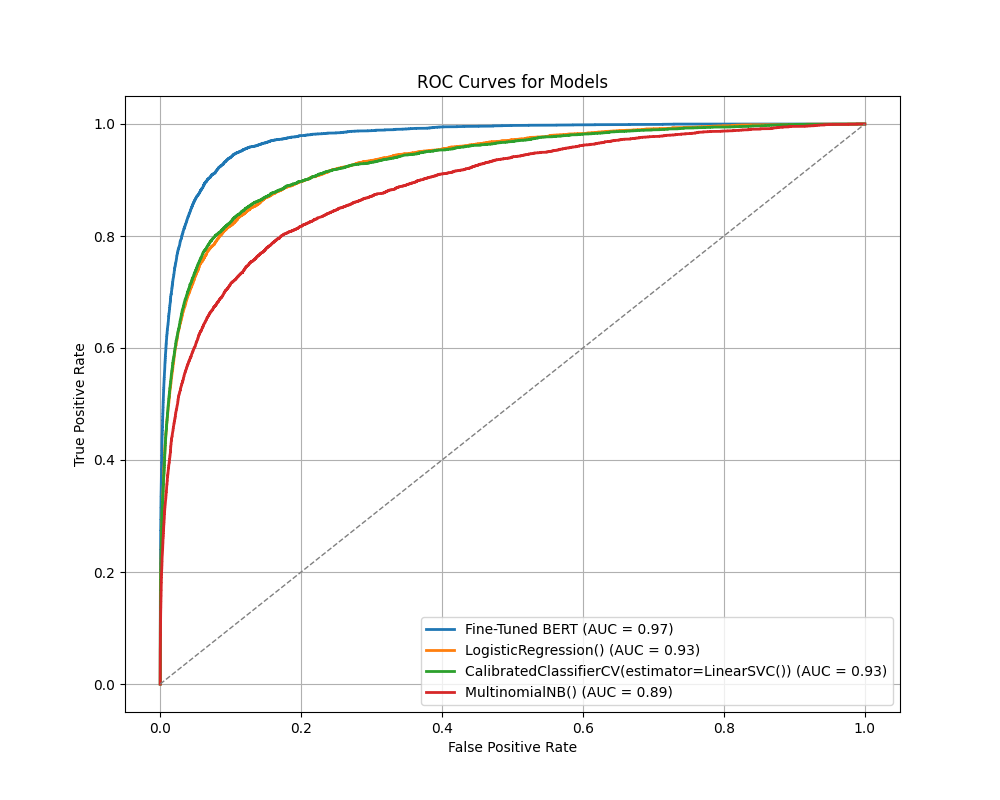
\includegraphics[width=0.7\textwidth]{./figures/combined_roc_curves.png}
    \caption{ROC Curves for BERT and baseline models}
    \label{fig:roc_curve_test_set}
\end{figure}